\documentclass[letterpaper,twoside]{article}
\usepackage{aistats2027}
\usepackage{amssymb,amsthm,mathtools,bm,microtype,enumitem,graphicx,booktabs}
\usepackage[colorlinks=true,linkcolor=blue,citecolor=blue,urlcolor=blue]{hyperref}
\usepackage[nameinlink,capitalize,noabbrev]{cleveref}
\newtheorem{theorem}{Theorem}[section]
\newtheorem{proposition}[theorem]{Proposition}
\newtheorem{lemma}[theorem]{Lemma}
\newtheorem{corollary}[theorem]{Corollary}
\theoremstyle{definition}
\newtheorem{definition}[theorem]{Definition}
\theoremstyle{remark}
\newtheorem{remark}[theorem]{Remark}

\newcommand{\R}{\mathbb R}
\newcommand{\N}{\mathbb N}
\newcommand{\cP}{\mathcal P}
\newcommand{\cM}{\mathcal M}
\newcommand{\supp}{\operatorname{supp}}
\newcommand{\spec}{\operatorname{spec}}
\newcommand{\diag}{\operatorname{diag}}
\newcommand{\Var}{\operatorname{Var}}
\newcommand{\ip}[2]{\langle #1,#2\rangle}
\newcommand{\norm}[1]{\lVert #1\rVert}
\newcommand{\doi}[1]{\href{https://doi.org/#1}{doi:#1}}


\hypersetup{pdftitle={Periodic Barzilai--Borwein Switching: Phase Balance and Exact Local Gaps},pdfauthor={}}
\makeatletter
\renewcommand{\Notice@String}{Research working paper. Author review pending.}
\makeatother
\begin{document}
\twocolumn[
\aistatstitle{Periodic Barzilai--Borwein Switching:\\Phase Balance and Exact Local Gaps}
\aistatsauthor{Research working paper}
\aistatsaddress{AI-assisted. Author review pending.}
]
\fancyhead[CE,CO]{\small\bfseries Research working paper}
\begin{abstract}
We study gradient methods that recompute a BB1 or BB2 stepsize at every iteration according to a prescribed periodic pattern. On positive definite quadratics with spectra in $[a,b]$, either fixed rule has sharp worst-case asymptotic gradient factor $C=(b-a)/(b+a)$. Every pattern using both rules has a strictly smaller uniform asymptotic threshold. Near condition number one, we determine the leading improvement: $C-Q_{\bm\sigma}=K_{\bm\sigma}C^3+O(C^4)$. Here $Q_{\bm\sigma}$ denotes either the supremum of the finite-dimensional trajectory factors or the threshold for a geometric bound uniform over all admissible finite-dimensional problems. The remainder is independent of the pattern and its period. The coefficient is half the variance of an explicit periodic linear response; alternation gives $K_{01}=1/32$. The proof characterizes equality at the spectral endpoints and estimates how the interior spectrum affects the worst-case factor near condition number one. Away from this limit, interior cycles can be slower than the endpoint construction. Numerical experiments compare the methods under a fixed iteration budget.
\end{abstract}

\section{Introduction}
Barzilai--Borwein steps estimate curvature from the most recent displacement and gradient difference. They require little storage and can produce rapid progress without line searches on positive quadratic objectives \cite{BarzilaiBorwein1988,Raydan1993,DaiLiao2002}. Their two classical forms are
\begin{equation}\label{eq:bb}
 \alpha_k^{\rm BB1}=\frac{s_{k-1}^{\mathsf T}s_{k-1}}{s_{k-1}^{\mathsf T}y_{k-1}},
 \qquad
 \alpha_k^{\rm BB2}=\frac{s_{k-1}^{\mathsf T}y_{k-1}}{y_{k-1}^{\mathsf T}y_{k-1}},
\end{equation}
where $s_{k-1}=x_k-x_{k-1}$ and $y_{k-1}=g_k-g_{k-1}$.
Over the class of Hessians with spectra in $[a,b]$, $0<a<b$, either fixed rule has sharp worst trajectory factor
\[
 C=\frac{b-a}{b+a}.
\]
This fixed-rule result is due to Yang and Yuan \cite{YangYuan2026}. The equality trajectory lives at the two spectral endpoints and uses the constant step $2/(a+b)$.

The extremal endpoint distributions of BB1 and BB2 are different. BB1 balances equal endpoint energies; BB2 balances the same energies after multiplication by the eigenvalue. This suggests a specific question: can a time-dependent rule preserve the common numerical step without preserving a common balancing distribution? On an endpoint spectrum, that step leaves all energy proportions unchanged. Switching therefore places incompatible demands on the same state. The difficulty is to turn this observation into a strict bound over \emph{all} spectra, including arbitrarily many interior eigenvalues and continuous spectrum.

Our main result is $C-Q_{\bm\sigma}=K_{\bm\sigma}C^3+O(C^4)$ as $C\downarrow0$, for both the supremal finite-dimensional trajectory factor and the uniform-envelope threshold, with a remainder bound independent of the finite word and period (\cref{cor:cubic}). The coefficient is half a periodic-response variance; $K_{01}=1/32$. The known endpoint recurrence \cite{DaiHuangLiu2019} supplies an explicit orbit. The main challenge is to prove its coefficient sharp over arbitrary spectra. Common endpoint balance also characterizes equality with $C$ and yields a strict gap for every mixed word throughout $0<C<1$ (\cref{thm:main}).

The algorithms themselves are established. Grippo and Sciandrone use safeguarded alternation \cite{GrippoSciandrone2002}; projected alternating BB gives explicit odd/even choices \cite{DaiFletcherProjected2005}. Cyclic BB repeats a computed step for a prescribed block \cite{DaiHagerSchittkowskiZhang2006}; adaptive selection and convex mixtures are developed in \cite{ZhouGaoDai2006,FrassoldatiZanniZanghirati2008,DaiHuangLiu2019}. Hilbert-space $R$-linear convergence under stepwise BB1/BB2 choice is already established \cite{AzmiKunisch2020}. Our question concerns their sharp asymptotic obstruction under a prescribed periodic \emph{selector} word. Each numerical step still depends on the observed gradient history. This differs from prescribing numerical steps, as in cyclical momentum \cite{GoujaudScieurDieuleveutTaylorPedregosa2022} and stepsize hedging \cite{AltschulerParrilo2025a}.

Gu \cite[Theorem~2.1]{Gu2026CSD} proves almost-everywhere doubly exponential convergence of cyclic steepest descent for a fixed finite-dimensional positive definite quadratic with $q$ distinct eigenvalues when $2j>q$. That method repeats a fresh cycle-start steepest-descent stepsize for $j$ updates. Gu also studies cyclic reuse of historical Ritz values in limited-memory steepest descent \cite{Gu2026Ritz}. Here we recompute a delayed BB stepsize at each update according to a periodic selector word and study worst-case thresholds over all admissible initializations and spectra.

The endpoint certificate and spectral-measure construction are inherited from the fixed-rule analysis \cite{YangYuan2026}. The subsequent Lyapunov formulation develops the endpoint defect \cite{YangYuanLyapunov2026}, while the closed-cone formulation identifies homogeneous growth with the envelope threshold \cite{YangYuanCone2026}. Here equality is resolved simultaneously across phases. The principal quantitative step is a second-order concentration estimate for arbitrary-spectrum maximizing measures, which identifies their local response with the endpoint recurrence. A stable inverse makes the remainder uniform over all periods.

The worst-trajectory factor takes the asymptotic root rate of each run and then the supremum over admissible runs. A uniform envelope requires a single prefactor for the bound relative to the first post-warm-up gradient, over all admissible problems and iteration numbers. We prove
\begin{equation}\label{eq:hierarchy}
 q^{\rm fd}_{\bm U}\le q^{\rm H}_{\bm U}
 =\Theta^{\rm fd}_{\bm U}=\Gamma_{\bm U}.
\end{equation}
Here finite-dimensional trajectory exactness, $q^{\rm fd}_{\bm U}=\Gamma_{\bm U}$, remains open for a general word. The equality for $\Theta^{\rm fd}_{\bm U}$ states that arbitrarily long finite-dimensional prefixes certify the threshold. It does not require one finite-dimensional trajectory to attain it.

\section{Periodic delayed spectral selectors}\label{sec:setting}
Let $\mathcal H$ be a real Hilbert space and
\[
\begin{gathered}
 q(x)=\tfrac12\langle Ax,x\rangle-\langle d,x\rangle,\\
 A=A^*,\qquad 0<aI\le A\le bI.
\end{gathered}
\]
Write $g_k=A(x_k-A^{-1}d)$. An arbitrary $\alpha_0>0$ produces $g_1=(I-\alpha_0A)g_0$.
For $g_k\ne0$, its scalar spectral probability is
\[
 \nu_k(B)=\frac{\langle E_A(B)g_k,g_k\rangle}{\|g_k\|^2}.
\]
Let $\mathcal P([a,b])$ carry the weak topology. A selector $U:\mathcal P([a,b])\to[a,b]$ is continuous and \emph{internal} when
\[
 \min\supp\nu\le U(\nu)\le\max\supp\nu.
\]
For a fixed period $L$ and selectors $\bm U=(U_0,\ldots,U_{L-1})$, use
\begin{equation}\label{eq:iteration}
\begin{gathered}
 g_{k+1}=\left(I-\frac{A}{U_j(\nu_{k-1})}\right)g_k,\\
 j=k-1\pmod L,\qquad k\ge1.
\end{gathered}
\end{equation}
Thus phase zero first updates $g_1$ using $g_0$. Finite termination is followed by zero extension. In this notation
\[
 U_0^{\rm BB}(\nu)=\int\lambda\,d\nu,\qquad
 U_1^{\rm BB}(\nu)=\frac{\int\lambda^2\,d\nu}{\int\lambda\,d\nu}.
\]
A binary word $\bm\sigma\in\{0,1\}^L$ chooses these selectors. The warm-up is called matched when $\alpha_0=1/U_0(\nu_0)$; matching is optional.

Define the trajectory factor
\[
 \rho_g=\limsup_{k\to\infty}
 \left(\frac{\|g_k\|}{\|g_1\|}\right)^{1/k},
\]
with value zero for finite termination, including $g_1=0$. The quantities $q^{\rm H}_{\bm U}$ and $q^{\rm fd}_{\bm U}$ are the suprema over the Hilbert and finite-dimensional problem classes, including initial gradients and positive warm-ups. The envelope threshold is
\begin{equation}\label{eq:threshold}
\begin{split}
 \Theta^{\rm fd}_{\bm U}
 =\inf\{\tau>0:\ &\exists K_\tau\ge1\ \ \forall A,g_0,\alpha_0,\ k\ge1,\\[-1mm]
 &\|g_k\|\le K_\tau\tau^{k-1}\|g_1\|\},
\end{split}
\end{equation}
where $A$ ranges over every finite dimension and the stated spectral interval. The prefactor may depend on $a,b,\bm U,\tau$, but on no instance parameter. An unrestricted positive warm-up requires normalization by $g_1$; it can make $\|g_1\|/\|g_0\|$ arbitrarily large.

\subsection{The normalized system}
For $u\in[a,b]$, set
\[
\begin{gathered}
 Q_u(\lambda)=(1-\lambda/u)^2,\quad R_u(w)=\int Q_u\,dw,\\
 F_uw=Q_uw/R_u(w)\qquad(R_u(w)>0).
\end{gathered}
\]
The normalized state contains the current and previous spectral probabilities and the phase:
\begin{align}
 T(w,z,j)&=(F_{U_j(z)}w,w,j+1),\label{eq:lift}\\
 f(w,z,j)&=\tfrac12\log R_{U_j(z)}(w).\nonumber
\end{align}
Adjoin an isolated terminal state $\theta$. States with $R_{U_j(z)}(w)=0$ map to $\theta$, which is fixed, and have $f=-\infty$. This compact metric state space has a Borel map $T$ continuous away from the terminal set $D$; $f$ is upper semicontinuous, bounded above, and $-\infty$ on $D$. For a nonterminal trajectory,
\begin{equation}\label{eq:cocycle-main}
 \log\frac{\|g_{n+1}\|}{\|g_1\|}
 =\sum_{t=0}^{n-1}f(T^t(\nu_1,\nu_0,0)).
\end{equation}
Let $\mathcal M_T$ be its invariant probabilities and define
\begin{equation}\label{eq:Gamma}
 \beta_{\bm U}=\sup_{\Pi\in\mathcal M_T}\int f\,d\Pi,
 \qquad \Gamma_{\bm U}=e^{\beta_{\bm U}},
\end{equation}
using $e^{-\infty}=0$. The integral is defined by decreasing lower truncations $f_M=\max(f,-M)$.

\section{A sharp phase-balance criterion}\label{sec:balance}
Put $m=(a+b)/2$ and
\[
 \mathcal B_j=\{p\in(0,1):U_j(p\delta_a+(1-p)\delta_b)=m\}.
\]
These sets depend only on how the selectors act on endpoint probabilities.

\begin{theorem}[Threshold and common balance]\label{thm:main}
For the continuous internal selectors in \cref{sec:setting}, \cref{eq:hierarchy} holds and $0\le\Gamma_{\bm U}\le C$. Moreover,
\begin{equation}\label{eq:balance-main}
 \Gamma_{\bm U}=C
 \quad\Longleftrightarrow\quad
 \bigcap_{j=0}^{L-1}\mathcal B_j\ne\varnothing.
\end{equation}
When equality holds, a two-dimensional endpoint orbit with matched warm-up $2/(a+b)$ attains $C$. For every $\tau>\Gamma_{\bm U}$ there is a finite $K_\tau$ such that the envelope in \cref{eq:threshold} holds also in Hilbert space.
\end{theorem}

For BB1, $\mathcal B_0=\{1/2\}$; for BB2, $\mathcal B_1=\{b/(a+b)\}$. They are disjoint. Thus every word containing both symbols has $\Gamma_{\bm\sigma}<C$. The strict gap depends on the word and spectral interval, and holds uniformly over all admissible warm-ups.

A broader example is a positive spectral weight,
\[
 U_j(\nu)=\frac{\int\lambda\Psi_j(\lambda)\,d\nu}
                  {\int\Psi_j(\lambda)\,d\nu},
 \qquad \Psi_j>0\ \text{continuous}.
\]
Its sole balancing mass is $\Psi_j(b)/(\Psi_j(a)+\Psi_j(b))$. Two distinct endpoint weight ratios are sufficient for a strict gap. Likewise, fixed convex combinations of the BB numerical steps \cite{DaiHuangLiu2019} retain $C$, whereas every nonconstant periodic mixing parameter has incompatible balance. The supplement proves this assertion, including uniqueness and monotonicity of the balancing mass.

\subsection{Why endpoint equality is rigid}
We give the principal argument; the supplement supplies the measure-theoretic details and full proofs.

\begin{lemma}[Persistent support and endpoint rigidity]\label{lem:rigidity}
Every ergodic invariant probability $\Pi$ with finite $f$-average has a deterministic compact support $S$ with at least two points, shared by both spectral coordinates almost surely. Its phase marginal is uniform. With $A_S=\min S$, $B_S=\max S$,
\[
 \int f\,d\Pi\le\log\frac{B_S-A_S}{B_S+A_S}\le\log C.
\]
Equality with $\log C$ forces $S=\{a,b\}$ and $U_j(z)=m$ almost surely.
\end{lemma}

\begin{proof}[Proof mechanism]
A normalized update cannot add spectral support. For each open set in a countable base, its positive-mass indicator is nonincreasing along $T$. Invariance makes it constant almost surely and ergodicity makes it deterministic. This gives the shared support; stationarity of the phase gives its uniform marginal.

For active endpoints $A_S,B_S$, write $p=B_S/(A_S+B_S)$ and $q=1-p$. The scalar inequality
\begin{equation}\label{eq:endpoint}
 \left(\frac{u-A_S}{u}\right)^p
 \left(\frac{B_S-u}{u}\right)^q
 \le\frac{B_S-A_S}{B_S+A_S}
\end{equation}
has equality only at the midpoint. Apply it first to narrow endpoint bands. Their negative log masses form a coboundary: each update bounds $f$ by a band version of the left-hand log in \cref{eq:endpoint}, plus the change in that coboundary. At recurrence times of a generic state, choose bands whose boundaries carry no initial mass. Their masses return, so the coboundary average vanishes along this subsequence. Shrinking the bands proves the inequality. Applying the same argument to bounded truncations of the nonnegative midpoint defect retains the equality information.

At equality, active endpoints must be $a,b$ and all reciprocal steps must be $m$. Then $R_m(w)\le C^2$, with equality only on $\{a,b\}$. Equality of its average forces endpoint support.
\end{proof}

At this midpoint step, $F_mw=w$ for every endpoint probability. Consequently an equality invariant measure lies on $w=z$, and its endpoint mass is invariant. Ergodicity fixes one mass $p$ across every phase. It must belong to all $\mathcal B_j$. Conversely any common mass gives an invariant endpoint orbit. This proves the equivalence once a maximal invariant measure is available.

\subsection{Compactness, realization, and the envelope}
The terminating boundary requires care because $T$ is not globally continuous. If invariant $\Pi_n$ have averages approaching a finite maximum and $\Pi_n\Rightarrow\Pi$, upper semicontinuity of every $f_M$ gives
\[
 \beta_{\bm U}\le\int f_M\,d\Pi\quad\text{for every }M.
\]
Hence $\int f\,d\Pi\ge\beta_{\bm U}>-\infty$, so $\Pi(D)=0$. The functions $\varphi\circ T$ are then continuous $\Pi$-almost everywhere for continuous $\varphi$. Passing invariance to the limit is legitimate. Ergodic decomposition supplies an ergodic maximizing measure.

The same truncation argument gives a semi-uniform bound in the spirit of Sturman and Stark \cite{SturmanStark2000}; the singular Borel-map form is proved in the supplement. If invariant averages are at most a finite $\beta$, then, for each $\varepsilon>0$,
\begin{equation}\label{eq:semi}
 \sum_{t=0}^{n-1}f(T^tx)\le n(\beta+\varepsilon)+B_\varepsilon
 \quad\text{for all }x,n.
\end{equation}
Indeed, a sequence of longer violating orbit segments has empirical measures with a weak limit of average exceeding $\beta$. Truncation again makes the discontinuity set null; telescoping $\varphi\circ T-\varphi$ proves invariance, a contradiction. Finite remaining lengths give $B_\varepsilon$. If $\beta_{\bm U}=-\infty$, apply this argument with every finite benchmark. This proves all envelope upper bounds.

For sharpness when $\Gamma_{\bm U}>0$, choose a maximizing generic state in phase $L-1$, say $(w,z,L-1)$, and put $u=U_{L-1}(z)$. Its successor is the compatible phase-zero pair $(F_uw,w,0)$. On the real space $L^2([a,b],w)$, let $A$ multiply by $\lambda$, $g_0=1$, and $\alpha_0=1/u$. This realizes that pair, and Birkhoff's theorem with \cref{eq:cocycle-main} gives $\rho_g=\Gamma_{\bm U}$. Thus $q^{\rm H}_{\bm U}=\Gamma_{\bm U}$.

Finally fix $0<\tau<\Gamma_{\bm U}$ and any proposed $K\ge1$. A sufficiently long regular prefix of this same orbit violates $K\tau^n$. Finite atomic probabilities $w_r\Rightarrow w$ approximate that prefix, because all finitely many normalizers are positive. Realizing each $w_r$ by a diagonal matrix and retaining the same warm-up gives a finite-dimensional violation. Hence $\Theta^{\rm fd}_{\bm U}\ge\Gamma_{\bm U}$. The approximating dimension can depend on prefix length, explaining precisely the hierarchy in \cref{eq:hierarchy}.

\begin{figure*}[t]
\centering
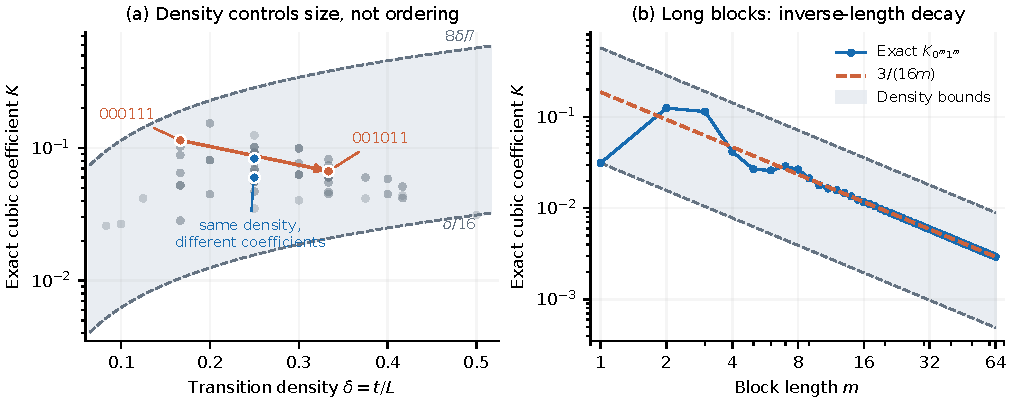
\includegraphics[width=\textwidth]{figures/exact_word_coefficients.pdf}
\caption{Exact cubic coefficients $K_{\bm\sigma}=V_{\bm\sigma}/2$ for $q^{\rm fd}_{\bm\sigma}$ and $\Gamma_{\bm\sigma}$ (Theorem~\ref{cor:cubic}): larger coefficients imply smaller factors near isotropy for fixed words. Left: 113 balanced primitive rotation classes through length 12 and proved density bounds. Highlighted words show unequal coefficients at equal density, and smaller coefficients despite more switches. Right: equal-block coefficients versus $3/(16m)$. These are exact formula evaluations, not trajectory estimates of $\Gamma$.}
\label{fig:mechanism}
\end{figure*}

\section{Quantitative gaps and an exact local law}\label{sec:gap}
The qualitative argument removes the fixed-rule equality orbit. The next result quantifies how far any invariant measure must stay from equality.

\begin{theorem}[Quantitative binary-word gap]\label{thm:quant}
Let $\bm\sigma$ contain both symbols and have period $L$. Let $t$ count its cyclic $1\to0$ boundaries and put $\ell=L/t\ge2$. Define
\begin{gather*}
 k_0=(1-C)^2/2,\quad H=(3-C)/(2(1-C)),\\
 Q_C=4+C/(1-C),\qquad B_\ell=2Q_C\ell,\\
 A_\ell=\frac{(14+C)\sqrt\ell+2Q_C\ell H}{\sqrt{k_0}},\\
 \delta_\ell(C)=\left(
 \frac{2C}{A_\ell+\sqrt{A_\ell^2+4C(B_\ell+C)}}\right)^2.
\end{gather*}
Then
\begin{equation}\label{eq:quant}
 0<\Gamma_{\bm\sigma}\le Ce^{-\delta_\ell(C)}<C.
\end{equation}
In particular, any $\tau$ strictly between $Ce^{-\delta_\ell(C)}$ and $C$ admits a uniform prefactor.
\end{theorem}

The certificate is conservative: for a fixed word,
\begin{equation}\label{eq:delta-regimes}
 \delta_\ell(C)\sim D_\ell C^2\ (C\downarrow0),\qquad
 \delta_\ell(C)\sim\frac{(1-C)^6}{8\ell^2}\ (C\uparrow1),
\end{equation}
where $D_\ell=[2(14\sqrt\ell+12\ell)^2]^{-1}$. It establishes full-spectrum separation but gives no computable prefactor. Averaging all $t$ boundaries improves the original length-based bound (recovered by using $L$) whenever $t>1$. The ratio $\ell=L/t$ is unchanged by repeating or rotating a word. This is a bound on the exact factor, not a rule for ordering exact factors of different words.

\begin{proof}[Quantitative mechanism]
Consider a finite-average ergodic invariant measure and normalize its active interval by $\lambda=m_S+d_Sx$, $-1\le x\le1$. Put $r=d_S/m_S\le C$,
\[
\begin{gathered}
 s=(U_j(z)-m_S)/d_S,\qquad\mu(w)=\int x\,dw,\\
 J(w)=1-\int x^2\,dw.
\end{gathered}
\]
Here $J$ measures interior spectral mass. If $\Delta=\log r-\int f\,d\Pi$, the endpoint-band argument gives
\[
\begin{gathered}
 \Delta\ge\mathbb E_\Pi\mathcal D_r(s),\\
 \begin{aligned}
 \mathcal D_r(s)={}&\log(1+rs)-\tfrac{1+r}{2}\log(1+s)\\
 &-\tfrac{1-r}{2}\log(1-s).
 \end{aligned}
\end{gathered}
\]
This is a binary relative entropy. Pinsker's inequality yields $\mathcal D_r(s)\ge k_0s^2$. Also
\[
\begin{aligned}
 f&=\log r+\tfrac12\log\!\int(x-s)^2dw-\log(1+rs)\\
 &\le\log r-\tfrac12J+H|s|.
\end{aligned}
\]
Consequently
\begin{equation}\label{eq:defects}
 \mathbb E_\Pi s^2\le\Delta/k_0,\qquad
 \mathbb E_\Pi J\le 2\Delta+2H\sqrt{\Delta/k_0}.
\end{equation}
Let $\Pi_j$ be the normalized phase-$j$ conditional, so $T_\#\Pi_j=\Pi_{j+1}$. For any set $I$ of $t$ distinct phases, conditional Cauchy--Schwarz and nonnegativity give
\[
\begin{aligned}
 \frac1t\sum_{j\in I}\mathbb E_{\Pi_j}|s|&\le\sqrt{\ell\Delta/k_0},\\
 \frac1t\sum_{j\in I}\mathbb E_{\Pi_j}J
 &\le\ell(2\Delta+2H\sqrt{\Delta/k_0}).
\end{aligned}
\]

The normalized BB selectors obey
\[
 s_0(w)=\mu(w),\qquad
 s_1(w)=\frac{\mu(w)+r(1-J(w))}{1+r\mu(w)}.
\]
Thus $|\mu+r|\le(1+C)|s_1|+C J/(1-C)$. A normalized update $w'\propto(x-\widehat s)^2w$ satisfies
\[
 |\mu(w')-\mu(w)|\le4(J(w)+3|\widehat s|).
\]
This follows by bounding the change of the multiplier from one, using the trivial mean bound when its normalizer is small.

At a cyclic BB2-to-BB1 boundary, the successive delayed selectors read $w$ and $w'$. Applying
\[
 r\le|\mu(w)+r|+|\mu(w')-\mu(w)|+|\mu(w')|
\]
at every boundary and then averaging gives $r\le A_\ell\sqrt\Delta+B_\ell\Delta$. Indeed, the three selector terms read phases $j,j-1,j+1$; each translated boundary set contains exactly $t$ distinct phases, so the displayed conditional bounds apply separately. Overlap between these three sets causes no additional assumption. If $G=\log C-\int f\,d\Pi$, then $\Delta\le G$ and $r\ge Ce^{-G}$. For $G<1$,
\[
 C\le A_\ell\sqrt G+(B_\ell+C)G.
\]
Solving this quadratic in $\sqrt G$ gives $G\ge\delta_\ell(C)$; $G\ge1$ is immediate since $\delta_\ell(C)<1$. Ergodic decomposition proves \cref{eq:quant}. Positivity follows from the endpoint response constructed next.
\end{proof}

\subsection{Exact endpoint response}
For $A=\diag(1,\kappa)$, put $h_{-1}=g_0$, $h_0=g_1$, and let symbol $\sigma_n$ use $h_{n-1}$ to update $h_n$. With both endpoint components nonzero, define their log energy ratio $\ell_n$. Direct substitution gives
\begin{equation}\label{eq:forced}
 \ell_{n+1}=\ell_n-2\ell_{n-1}+2\sigma_n\log\kappa.
\end{equation}
This specializes the known spectral-gradient recurrence \cite{DaiHuangLiu2019}. The homogeneous eigenvalues are $(1\pm i\sqrt7)/2$, both of modulus $\sqrt2$. Hence there is a unique $L$-periodic solution $\ell_n=a_n\log\kappa$, determined by
\[
 a_{n+1}-a_n+2a_{n-1}=2\sigma_n,\qquad a_{n+L}=a_n.
\]
Put $r_n=1-a_{n-1}+\sigma_n$. Summing the recurrence gives $L^{-1}\sum r_n=1$.

\begin{proposition}[Endpoint response]\label{prop:two}
The periodic response is repelling, realizable by a positive warm-up, and has factor
\begin{equation}\label{eq:rho}
 \rho_{\bm\sigma}(\kappa)
 =\frac{\kappa-1}
 {\left[\prod_{n=0}^{L-1}(1+\kappa^{r_n})\right]^{1/L}}.
\end{equation}
It satisfies $\rho_{\bm\sigma}\le q^{\rm fd}_{\bm\sigma}\le\Gamma_{\bm\sigma}$. Every other full-support two-point projective pair has root factor zero. For a nonconstant word, $\rho_{\bm\sigma}<C$.
\end{proposition}

Over one period the endpoint multipliers have equal absolute products, giving \cref{eq:rho}. Strict convexity of $\log(1+\kappa^r)$ and the mean-one identity give strict separation. The zero-factor alternative follows because every window of a sufficiently large fixed length of a nonzero solution of the homogeneous recurrence contains positive and negative excursions of order $2^{n/2}$. Each excursion contracts one endpoint component; their products decay faster than exponentially. The supplement gives the complete window argument and treats disappearing components.

A desired pair of positive endpoint ratios $\zeta_{-1},\zeta_0$ is realized by $\alpha_0=(1+v)/(1+\kappa v)$, where $v=\sqrt{\zeta_0/\zeta_{-1}}$. This warm-up is generally unmatched. For $01$ the exceptional periodic pair cannot be reached by a phase-matched warm-up.

\subsection{The exact unrestricted local coefficient}
The endpoint response determines more than a lower bound near isotropy. Its leading gap is sharp over arbitrary spectra.

\begin{theorem}[Uniform exact cubic coefficient]\label{cor:cubic}
For a finite binary word, let $a_n,r_n$ be its periodic response and put
\[
 K_{\bm\sigma}=\frac{V_{\bm\sigma}}2
 =\frac1{2L}\sum_{n=0}^{L-1}(r_n-1)^2.
\]
For either $Q_{\bm\sigma}=q^{\rm fd}_{\bm\sigma}$ or $Q_{\bm\sigma}=\Gamma_{\bm\sigma}$,
\begin{equation}\label{eq:exact-cubic-main}
 C-Q_{\bm\sigma}=K_{\bm\sigma}C^3+O(C^4),
 \qquad C\downarrow0,
\end{equation}
where the remainder is uniform over all finite words and periods. More explicitly, its absolute value is at most $6400C^4$ for $0<C\le1/4$. Thus the word may depend on $C$.
\end{theorem}

\begin{proof}[Proof mechanism]
Write $(Sv)_j=v_{j+1}$ and $B=S-I+2S^{-1}$ on cyclic sequences. With $\zeta=(1+i\sqrt7)/4$,
\[
 B^{-1}=\sum_{k\ge1}h_kS^k,\qquad
 h_k=\frac2{\sqrt7}\operatorname{Im}\zeta^k.
\]
Since $\sum|h_k|<2$, the inverse is bounded uniformly in both the maximum norm and normalized $\ell^1$ norm, independently of the period. Since $Ba=2\bm\sigma$, the response $q_j=r_j-1$ is uniformly bounded. The endpoint product gives
\[
 \log(C/\rho_{\bm\sigma})=K_{\bm\sigma}C^2+O(C^4)
\]
with a uniform error. Take an ergodic maximizing measure for $\Gamma$, with active-hull variables $r,s,\mu,J$. Put $G=\log(C/\Gamma)$ and $\Delta=\log(r/\Gamma)$. The endpoint bounds give $0\le\Delta\le G=O(C^2)$ and $r=C+O(C^3)$. The defect and selector identities imply $\mathbb E s^2,\mathbb E\mu^2=O(C^2)$.

Retaining the cross term in
\[
 f-\log r\le-\tfrac12J-s\mu+\tfrac12s^2
                  +\frac r{1-r}|s|
\]
then gives $\mathbb EJ=O(C^2)$. The global update estimate
\[
 |\mu(w')-\mu(w)+2s|
 \le8(J+\mu^2)+12s^2
\]
also holds near zero normalizers. Let $M_j=\mathbb E_{\Pi_j}\mu(w)$ and $S_j=\mathbb E_{\Pi_j}s$. The phase equations are
\[
 M_{j+1}=M_j-2S_j+e_j,\qquad
 S_j=M_{j-1}+r\sigma_j+\eta_j,
\]
with $L^{-1}\sum|e_j|=O(C^2)$ and $L^{-1}\sum|\eta_j|=O(C^3)$. Applying the uniform inverse gives
\[
 \frac1L\sum_j|S_j-Cq_j|=O(C^2).
\]
No individual phase bound is needed. The inequality
$S_j^2\ge2Cq_jS_j-C^2q_j^2$ and the uniform bound on $q$ imply $L^{-1}\sum S_j^2\ge V_{\bm\sigma}C^2-O(C^3)$. Conditional Jensen in the endpoint defect yields
\[
 G\ge\Delta\ge\frac{(1-C)^2}{2L}\sum_jS_j^2
       \ge K_{\bm\sigma}C^2-O(C^3).
\]
The endpoint upper bound on $G$, followed by exponentiation, proves the uniform expansion for $\Gamma$. The sandwich $\rho\le q^{\rm fd}\le\Gamma$ proves the same for $q^{\rm fd}$. Supplement Section S15 tracks all constants.
\end{proof}

The coefficient measures the frequency content of the word. For
$\widehat\sigma_k=L^{-1}\sum_j\sigma_j e^{-2\pi i kj/L}$ and $\omega_k=2\pi k/L$,
\begin{equation}\label{eq:fourier-main}
 V_{\bm\sigma}=\sum_{k=1}^{L-1}
 \frac{1-\cos\omega_k}{1-3\cos\omega_k+4\cos^2\omega_k}
 |\widehat\sigma_k|^2.
\end{equation}
For mixed words, $1/(16\ell)\le V_{\bm\sigma}/2\le8/(7\ell)$, with the lower bound attained by alternation. Transition count alone does not order the exact local gaps: $000111$ has $t=1$ and coefficient $11/96$, whereas $001011$ has $t=2$ and the smaller coefficient $15/224$. Hence the former has the smaller unrestricted factor for all sufficiently small positive $C$. These compare asymptotic factors; the supplement gives a conservative explicit range, not a finite-budget ranking. For growing equal blocks $0^m1^m$, $K=3/(16m)+O(2^{-m/2}/m)$. Thus $C-Q\sim3C^3/(16m)$ jointly when $m\to\infty$ and $mC\to0$. The absolute uniform remainder does not imply a relative approximation for arbitrary growing words.

\section{Why interior spectrum matters}\label{sec:interior}
For alternation,
\[
\begin{gathered}(r_0,r_1)=(3/4,5/4),\\
 \rho_{01}(\kappa)=
 \frac{\kappa-1}{\sqrt{(1+\kappa^{3/4})(1+\kappa^{5/4})}}.
\end{gathered}
\]
Its endpoint gap has cubic coefficient $1/32$. At large $\kappa$, however, endpoint analysis misses a slower three-point orbit.

\begin{theorem}[An interior alternating cycle]\label{thm:three}
Let $\kappa=b/a>\kappa_*:=577+408\sqrt2$. On the spectrum $\{a,(a+b)/2,b\}$ an exact phase-period-two alternating cycle exists with factor
\[
 \rho_3(C)=\frac{C}{\sqrt{2-C^2}},\qquad
 \rho_{01}(\kappa)<\rho_3(C)\le\Gamma_{01}<C.
\]
It is realizable by an explicit unmatched positive warm-up.
\end{theorem}

The reciprocal steps are $u_0=m-d/\sqrt2$ and $u_1=m+d/\sqrt2$, where $d=(b-a)/2$. This pair and the resulting factor agree algebraically with the symmetric three-point construction in cyclic BB \cite[eqs.~(3.21)--(3.23)]{DaiHagerSchittkowskiZhang2006}. The additional issue here is compatibility with the \emph{alternating BB1 and BB2 quotients}.

To see this, write $\lambda=m+dx$, $x\in\{-1,0,1\}$ and $t=1/\sqrt2$. The phase-zero masses $p_x$ solve
\begin{equation}\label{eq:three-moments}
\begin{gathered}
 \sum p_x=1,\qquad \sum p_x(x+t)^3=0,\\
 \sum p_x(C^{-1}+x)(x-t)=0.
\end{gathered}
\end{equation}
The middle mass is
\[
 p_0=\frac{17C-12\sqrt2}{2(8C-3\sqrt2)}.
\]
All masses are positive exactly when $C>12\sqrt2/17$, equivalent to $\kappa>\kappa_*$. The second and third equations in \cref{eq:three-moments} enforce BB1 after the first reweighting and BB2 on the initial measure. Since $(x-t)(x+t)=\pm1/2$ on these nodes, the two-step squared multiplier is constant and closes the cycle. Starting from the phase-one probability and using $\alpha_0=1/u_1$ realizes it.

This construction also bounds what switching can achieve at large condition number. For $Q=q^{\rm fd}_{01}$ or $\Gamma_{01}$,
\begin{equation}\label{eq:large-kappa}
 2\le\liminf_{\kappa\to\infty}\kappa(1-Q)
 \le\limsup_{\kappa\to\infty}\kappa(1-Q)\le4.
\end{equation}
Indeed, $\rho_3=(\kappa-1)/\sqrt{\kappa^2+6\kappa+1}\le Q<C$ and the two bounds have deficits asymptotic to $4/\kappa$ and $2/\kappa$. The full-spectrum worst factor therefore retains the order $1-\Theta(\kappa^{-1})$, despite the endpoint response's $1-\Theta(\kappa^{-3/4})$ behavior.

The supplement determines the largest factor within the exact phase-period-two class with prescribed active extrema. Equal absolute two-step multipliers force support on at most four nodes and reciprocal steps symmetric about the active midpoint. The maximal factor is the endpoint response below and at $\kappa_*$, and the three-point factor above it. Higher-period and aperiodic maximizing measures remain possible.

\begin{figure*}[t]
\centering
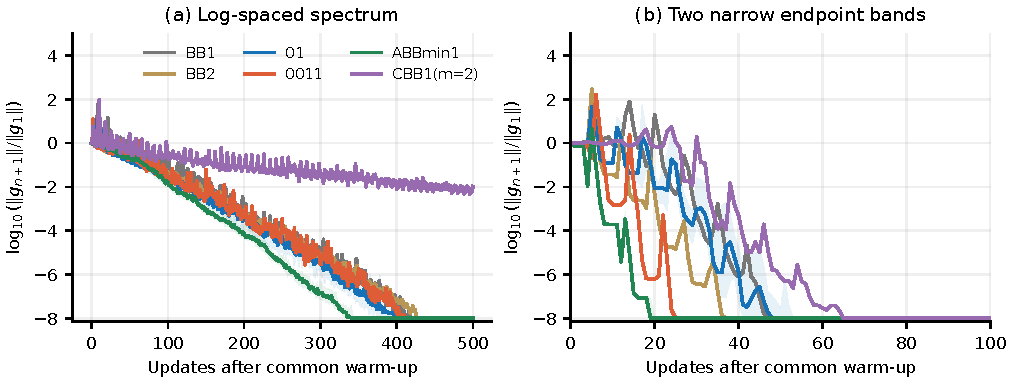
\includegraphics[width=\textwidth]{figures/finite_budget.pdf}
\caption{Finite budgets at $\kappa=1000$. Lines show median log gradient ratios across 20 common starts; shading shows the interquartile ranges for $01$ and ABBmin1 (linearly interpolated sample percentiles). Curves are held at $-8$ after first reaching the target, a reporting floor rather than exact termination. Nonmonotone excursions are retained. Equal update counts correspond to equal gradient-evaluation counts; selector inner products differ as stated in the text.}
\label{fig:budget}
\end{figure*}

\section{Controlled numerical evidence}\label{sec:experiments}

We check one complete delayed endpoint cycle at 90-digit precision for five words and seven condition numbers. Projective closure and relative factor errors are below $10^{-70}$. Figure~\ref{fig:mechanism} displays exact coefficients from rational periodic responses; the supplement retains the gap and interior-cycle plots. At $\kappa=2000$, the three-point factor is $0.998003991$, larger than the endpoint factor $0.997795863$. Its selector identities, closure, and specified unmatched warm-up are verified separately. Long floating-point runs cannot reliably trace a repelling response: for $01$ at $\kappa=100$, double precision produces a log energy-ratio error exceeding $0.01$ after 92 updates. The code retains this diagnostic.

For finite budgets we use 64-dimensional log-spaced, linearly spaced, and two-band spectra, $\kappa\in\{10,100,1000\}$, and 20 Gaussian initial gradients for each spectrum. The bands are $[1,1.05]$ and $[0.95\kappa,\kappa]$, with 32 nodes each. All methods use the same warm-up $\alpha_0=2/(1+\kappa)$, the specified one-step delay, and at most 500 subsequent updates. The target is $\|g_{n+1}\|/\|g_1\|\le10^{-8}$. No word or parameter search is performed on these 180 instances.

We compare BB1, BB2, $01$, $0011$, ABBmin1, and BB1 reuse with the prescribed cycle length two, denoted CBB1($m=2$). ABBmin1 uses the original rule with $\tau=0.8$ and $m=9$ \cite[eq.~(14)]{FrassoldatiZanniZanghirati2008}: when the BB2/BB1 ratio is below $\tau$, select the smallest BB2 value among the current and up to nine preceding values; otherwise use BB1. Normalized log spectral weights avoid absolute-gradient underflow. An independent signed-gradient implementation using actual secants agrees over the first 12 updates within $2.94\,10^{-14}$ in $\log_{10}$ norm ratio.

\begin{table}[t]
\centering
\caption{Median updates after warm-up to the target at $\kappa=1000$; 20 starts per cell. Timeouts are censored, not replaced by 500.}
\label{tab:budget}
\begin{tabular}{lrrr}
\toprule
Method & Log-spaced & Linear & Two bands\\
\midrule
BB1 &416.5&376.5&47\\
BB2 &426&386.5&37\\
$01$ &401&377.5&48\\
$0011$ &408.5&370.5&25\\
ABBmin1 &341&152&19\\
CBB1($m=2$) &$>500$&$>500$&63\\
\bottomrule
\end{tabular}
\end{table}



A budget of $n$ updates uses $n+2$ gradient evaluations including initialization. Under direct-secant accounting, selector inner products number $2n$ for either fixed rule or word, $3n$ for ABBmin1, and $2\lceil n/2\rceil$ for CBB1($m=2$). Norm monitoring is a common additional inner product; no function values or line searches are used. These counts recompute the secant quadratic forms directly. Fused inner products and cached monitoring norms change additional computation and communication costs. The diagonal simulator is not a wall-clock comparison. At $\kappa=1000$ on log-spaced spectra, the median $01$ and ABBmin1 costs are respectively 401 versus 341 updates, but 802 versus 1023 selector inner products.

All 43 timeouts among 1,080 runs are retained: 38 belong to CBB1($m=2$) and five to BB1, BB2, or $01$ on log-spaced $\kappa=1000$ instances. The corresponding solved counts are 19, 17, and 19 of 20 for BB1, BB2, and $01$. The supplement gives every initial condition, raw trace, seed, and censoring rule. Table~\ref{tab:budget} and Figure~\ref{fig:budget} show that alternation can be slower than BB1 at a finite budget, and ABBmin1 has the smallest displayed medians. These results test the scope of the asymptotic theorem rather than establish a general optimizer ranking.

\newpage
\section{Discussion}\label{sec:discussion}
The phase-balance condition explains the strict gap for a pattern that uses both BB rules: endpoint energies that give equality for one rule cannot give equality for the other. The quantitative bound averages over the switch points. Near condition number one, the endpoint construction gives the exact cubic coefficient for both the uniform threshold and the worst finite-dimensional trajectory factor. The coefficient depends on the full pattern. The remainder estimate is uniform over periods, although a relative asymptotic formula for a growing period also needs control of the coefficient. Away from this limit, interior cycles can be slower than the endpoint response.

The remaining questions concern the size and practical use of the gap: whether finite-dimensional worst trajectories attain $\Gamma$, which invariant measures maximize it, and how to compute a useful all-spectrum prefactor. A large prefactor is unavoidable even for two nodes. With $A=\diag(1,\kappa)$, $g_0=(1,\varepsilon)$ with $\varepsilon>0$, $\alpha_0=1$, and a first BB1 step,
\[
 \frac{\|g_2\|}{\|g_1\|}
 =\frac{\kappa-1}{1+\kappa\varepsilon^2}\longrightarrow\kappa-1.
\]
Thus any envelope at rate $\tau$ requires $K_\tau\ge(\kappa-1)/\tau$, despite subsequent termination.

\clearpage
\section*{AI Use Statement}
Generative AI assisted with the mathematical analysis, literature comparison, computation, and editing. Separate AI-assisted reviews examined the proofs, numerical records, and attribution. This public working version is based on the E01 manuscript. Final verification by the author is pending.

\begin{thebibliography}{99}
\raggedright
\bibitem{AltschulerParrilo2025a}
J.~M. Altschuler and P.~A. Parrilo.
Acceleration by stepsize hedging: Multi-step descent and the silver
stepsize schedule.
\emph{Journal of the ACM}, 72(2):Article 12, 1--38, 2025.
\doi{10.1145/3708502}.


\bibitem{AzmiKunisch2020}
B.~Azmi and K.~Kunisch.
Analysis of the Barzilai--Borwein step-sizes for problems in Hilbert spaces.
\emph{Journal of Optimization Theory and Applications}, 185(3):819--844, 2020.
\doi{10.1007/s10957-020-01677-y}.

\bibitem{BarzilaiBorwein1988}
J.~Barzilai and J.~M. Borwein.
Two-point step size gradient methods.
\emph{IMA Journal of Numerical Analysis}, 8(1):141--148, 1988.
\doi{10.1093/imanum/8.1.141}.


\bibitem{DaiFletcherProjected2005}
Y.-H.~Dai and R.~Fletcher.
Projected Barzilai--Borwein methods for large-scale box-constrained quadratic programming.
\emph{Numerische Mathematik}, 100:21--47, 2005.
\doi{10.1007/s00211-004-0569-y}.


\bibitem{DaiHagerSchittkowskiZhang2006}
Y.-H.~Dai, W.~W.~Hager, K.~Schittkowski, and H.~Zhang.
The cyclic Barzilai--Borwein method for unconstrained optimization.
\emph{IMA Journal of Numerical Analysis}, 26:604--627, 2006.
\doi{10.1093/imanum/drl006}.


\bibitem{DaiHuangLiu2019}
Y.-H.~Dai, Y.~Huang, and X.-W.~Liu.
A family of spectral gradient methods for optimization.
\emph{Computational Optimization and Applications}, 74:43--65, 2019.
\doi{10.1007/s10589-019-00107-8}.


\bibitem{DaiLiao2002}
Y.-H.~Dai and L.-Z.~Liao.
$R$-linear convergence of the Barzilai and Borwein gradient method.
\emph{IMA Journal of Numerical Analysis}, 22(1):1--10, 2002.
\doi{10.1093/imanum/22.1.1}.


\bibitem{FrassoldatiZanniZanghirati2008}
G.~Frassoldati, L.~Zanni, and G.~Zanghirati.
New adaptive stepsize selections in gradient methods.
\emph{Journal of Industrial and Management Optimization}, 4:299--312, 2008.
\doi{10.3934/jimo.2008.4.299}.


\bibitem{GoujaudScieurDieuleveutTaylorPedregosa2022}
B.~Goujaud, D.~Scieur, A.~Dieuleveut, A.~B. Taylor, and F.~Pedregosa.
Super-acceleration with cyclical step-sizes.
In \emph{Proceedings of the 25th International Conference on Artificial
Intelligence and Statistics}, volume 151 of \emph{Proceedings of Machine
Learning Research}, pages 3028--3065, 2022.


\bibitem{GrippoSciandrone2002}
L.~Grippo and M.~Sciandrone.
Nonmonotone globalization techniques for the Barzilai--Borwein gradient method.
\emph{Computational Optimization and Applications}, 23:143--169, 2002.
\doi{10.1023/A:1020587701058}.


\bibitem{Raydan1993}
M.~Raydan.
On the Barzilai and Borwein choice of steplength for the gradient method.
\emph{IMA Journal of Numerical Analysis}, 13(3):321--326, 1993.
\doi{10.1093/imanum/13.3.321}.


\bibitem{SturmanStark2000}
R.~Sturman and J.~Stark.
Semi-uniform ergodic theorems and applications to forced systems.
\emph{Nonlinearity}, 13(1):113--143, 2000.
\doi{10.1088/0951-7715/13/1/306}.


\bibitem{YangYuan2026}
S.~Yang and Y.-X.~Yuan.
The sharp worst-case asymptotic rate of the Barzilai--Borwein method in
$\R^d$ and Hilbert spaces.
arXiv:2608.07839, 2026.
\doi{10.48550/arXiv.2608.07839}.


\bibitem{ZhouGaoDai2006}
B.~Zhou, L.~Gao, and Y.-H.~Dai.
Gradient methods with adaptive step-sizes.
\emph{Computational Optimization and Applications}, 35:69--86, 2006.
\doi{10.1007/s10589-006-6446-0}.


\bibitem{YangYuanLyapunov2026}
S.~Yang and Y.-X.~Yuan.
Lyapunov functions and $R$-linear convergence for quadratic
Barzilai--Borwein dynamics.
arXiv:2609.12084, 2026.
\url{https://arxiv.org/abs/2609.12084}.


\bibitem{YangYuanCone2026}
S.~Yang and Y.-X.~Yuan.
$R$-linear convergence of Barzilai--Borwein methods on strictly convex
quadratics via closed-cone homogeneous dynamics.
arXiv:2609.12100, 2026.
\url{https://arxiv.org/abs/2609.12100}.


\bibitem{Gu2026CSD}
R.~Gu.
Doubly exponential convergence of the cyclic steepest descent method
for strictly convex quadratics in arbitrary dimensions.
arXiv:2609.25800v1, 2026.
\url{https://arxiv.org/abs/2609.25800v1}.

\bibitem{Gu2026Ritz}
R.~Gu.
Superlinear convergence of cyclic gradient methods with historical Ritz step sizes.
arXiv:2610.32705v2, 2026.
\url{https://arxiv.org/abs/2610.32705v2}.

\end{thebibliography}


\section*{Checklist}
\begin{enumerate}
\item For all models and algorithms presented, check if you include:
\begin{enumerate}
\item A clear description of the mathematical setting, assumptions, algorithm, and/or model. [Yes; Section~\ref{sec:setting}.]
\item An analysis of the properties and complexity (time, space, sample size) of any algorithm. [Yes; asymptotic factors and selector costs, Sections~\ref{sec:balance}--\ref{sec:experiments}.]
\item (Optional) Anonymized source code, with specification of all dependencies, including external libraries. [Yes; supplementary ZIP.]
\end{enumerate}
\item For any theoretical claim, check if you include:
\begin{enumerate}
\item Statements of the full set of assumptions of all theoretical results. [Yes; statements in the main text and supplement.]
\item Complete proofs of all theoretical results. [Yes; detailed proofs in the supplement.]
\item Clear explanations of any assumptions. [Yes; Section~\ref{sec:setting} and initialization discussion.]
\end{enumerate}
\item For all figures and tables that present empirical results, check if you include:
\begin{enumerate}
\item The code, data, and instructions needed to reproduce the main experimental results (either in the supplemental material or as a URL). [Yes; supplementary ZIP.]
\item All the training details (e.g., data splits, hyperparameters, how they were chosen). [Yes; no training; fixed experimental parameters in Section~\ref{sec:experiments} and supplementary README.]
\item A clear definition of the specific measure or statistics and error bars (e.g., with respect to the random seed after running experiments multiple times). [Yes; Figure~\ref{fig:budget} and supplementary protocol.]
\item A description of the computing infrastructure used. (e.g., type of GPUs, internal cluster, or cloud provider). [Yes; local CPU, Python and library versions in supplementary environment file.]
\end{enumerate}
\item If you are using existing assets (e.g., code, data, models) or curating/releasing new assets, check if you include:
\begin{enumerate}
\item Citations of the creator If your work uses existing assets. [Yes; mathematical and algorithmic sources cited.]
\item The license information of the assets, if applicable. [No; code licensing decision remains for the author before public release.]
\item New assets either in the supplemental material or as a URL, if applicable. [Yes; code and generated data.]
\item Information about consent from data providers/curators. [Not Applicable; synthetic quadratic instances.]
\item Discussion of sensible content if applicable, e.g., personally identifiable information or offensive content. [Not Applicable.]
\end{enumerate}
\item If you used crowdsourcing or conducted research with human subjects, check if you include:
\begin{enumerate}
\item The full text of instructions given to participants and screenshots. [Not Applicable.]
\item Descriptions of potential participant risks, with links to Institutional Review Board (IRB) approvals if applicable. [Not Applicable.]
\item The estimated hourly wage paid to participants and the total amount spent on participant compensation. [Not Applicable.]
\end{enumerate}
\end{enumerate}
\end{document}

